\chapter{Brownian Motion, Diffusion, and the Heat Equation}
\label{ch:brownian-motion-diffusion}

Transport describes the redistribution of particles, charge, energy, or another
conserved quantity.  A microscopic trajectory is irregular, while an ensemble
of trajectories has reproducible moments and a deterministic density.
This chapter derives the diffusion equation from a random walk, formulates the
same limit as a stochastic differential equation, constructs Fick's law from
particle crossings, and develops the matrix exponential used to propagate a
discretized diffusion equation.  The final sections apply these results to
electron and hole currents in semiconductors.

The derivation follows the transport sequence of Sze and Lee
\cite[Chap.~2]{szeLee2012} and the distribution-function hierarchy developed by
Rudan \cite[Chaps.~6 and 19]{rudan2015}.  The stochastic formulation uses the
Wiener and It\^o framework \cite{wiener1923,ito1944}.

\section{The random-walk limit}

Consider a one-dimensional walker whose independent increments have duration
$\Delta t$ and values
\begin{equation}
  \Delta X_s=
  \begin{cases}
    +\ell,&\text{with probability }1/2,\\
    -\ell,&\text{with probability }1/2.
  \end{cases}
  \label{eq:transport-random-step}
\end{equation}
The first two moments are
\begin{equation}
  \langle\Delta X_s\rangle=0,
  \qquad
  \langle\Delta X_s\Delta X_{s'}\rangle
  =\ell^2\delta_{ss'}.
  \label{eq:transport-step-moments}
\end{equation}
After $N$ steps,
\begin{equation}
  X_N-X_0=\sum_{s=1}^{N}\Delta X_s.
  \label{eq:transport-position-sum}
\end{equation}
Independence removes the cross terms in the second moment, so
\begin{equation}
  \left\langle X_N-X_0\right\rangle=0,
  \qquad
  \left\langle(X_N-X_0)^2\right\rangle=N\ell^2.
  \label{eq:transport-random-walk-msd}
\end{equation}
Writing $t=N\Delta t$ and defining
\begin{equation}
  D=\frac{\ell^2}{2\Delta t}
  \label{eq:transport-random-walk-diffusivity}
\end{equation}
gives the one-dimensional mean-square-displacement law
\begin{equation}
  \boxed{\left\langle(X(t)-X_0)^2\right\rangle=2Dt.}
  \label{eq:transport-one-dimensional-msd}
\end{equation}
For isotropic diffusion in $d$ dimensions,
\begin{equation}
  \boxed{
  \left\langle|\bm R(t)-\bm R_0|^2\right\rangle=2dDt.
  }
  \label{eq:transport-dimensional-msd}
\end{equation}
The linear dependence on time defines normal diffusion.  Motion with a
persistent velocity is ballistic and has a mean-square displacement
proportional to $t^2$ at short times.

The diffusion limit requires observation lengths much larger than $\ell$ and
observation times much longer than $\Delta t$.  Correlated increments, broad
waiting-time distributions, and long jumps produce transport laws that do not
reduce to \cref{eq:transport-dimensional-msd}.

\section{Brownian motion and drift--diffusion dynamics}

A Wiener process $\bm W_t$ has independent Gaussian increments with
\begin{equation}
  \mathbb E[\dd\bm W_t]=\bm 0,
  \qquad
  \mathbb E[\dd\bm W_t\dd\bm W_t^{\mathsf T}]
  =I\,\dd t.
  \label{eq:transport-wiener-increments}
\end{equation}
The It\^o stochastic differential equation
\begin{equation}
  \dd\bm R_t
  =\bm b(\bm R_t,t)\,\dd t
  +B(\bm R_t,t)\,\dd\bm W_t
  \label{eq:transport-general-sde}
\end{equation}
contains a deterministic drift velocity $\bm b$ and stochastic increments with
diffusion tensor
\begin{equation}
  \bm D=\frac12BB^{\mathsf T}.
  \label{eq:transport-diffusion-tensor}
\end{equation}
For constant isotropic diffusion, $B=\sqrt{2D}\,I$ and
\begin{equation}
  \dd\bm R_t=\bm b\,\dd t+\sqrt{2D}\,\dd\bm W_t.
  \label{eq:transport-isotropic-sde}
\end{equation}
Its ensemble moments are
\begin{equation}
  \mathbb E[\bm R_t]=\bm R_0+\bm b t,
  \qquad
  \operatorname{Cov}(\bm R_t)=2Dt\,I.
  \label{eq:transport-sde-moments}
\end{equation}
Drift controls the mean position.  Diffusion controls spreading about that
mean.  The uncentered second moment contains both contributions and therefore
cannot be used as a diffusion estimate when $\bm b\ne\bm0$.

For a smooth scalar function $f(\bm R,t)$, It\^o's formula gives
\begin{equation}
\begin{aligned}
  \dd f={}&
  \left[
    \frac{\partial f}{\partial t}
    +\bm b\cdot\nabla f
    +\sum_{ij}D_{ij}\frac{\partial^2f}{\partial x_i\partial x_j}
  \right]\dd t
  +(\nabla f)^{\mathsf T}B\,\dd\bm W_t.
\end{aligned}
  \label{eq:transport-ito-formula}
\end{equation}
The second-derivative term is the It\^o correction.  It converts stochastic
path dynamics into diffusion of the ensemble density.

A direct numerical approximation is the Euler--Maruyama update
\begin{equation}
  \bm R_{r+1}
  =\bm R_r+\bm b(\bm R_r,t_r)\Delta t
  +B(\bm R_r,t_r)\sqrt{\Delta t}\,\bm\eta_r,
  \label{eq:transport-euler-maruyama}
\end{equation}
where the components of $\bm\eta_r$ are independent standard normal random
variables.  Independent particles require independent random vectors.
Convergence must be checked by reducing $\Delta t$ and increasing the ensemble
size \cite{higham2001,kloedenPlaten1992}.

\begin{figure}[htbp]
  \centering
  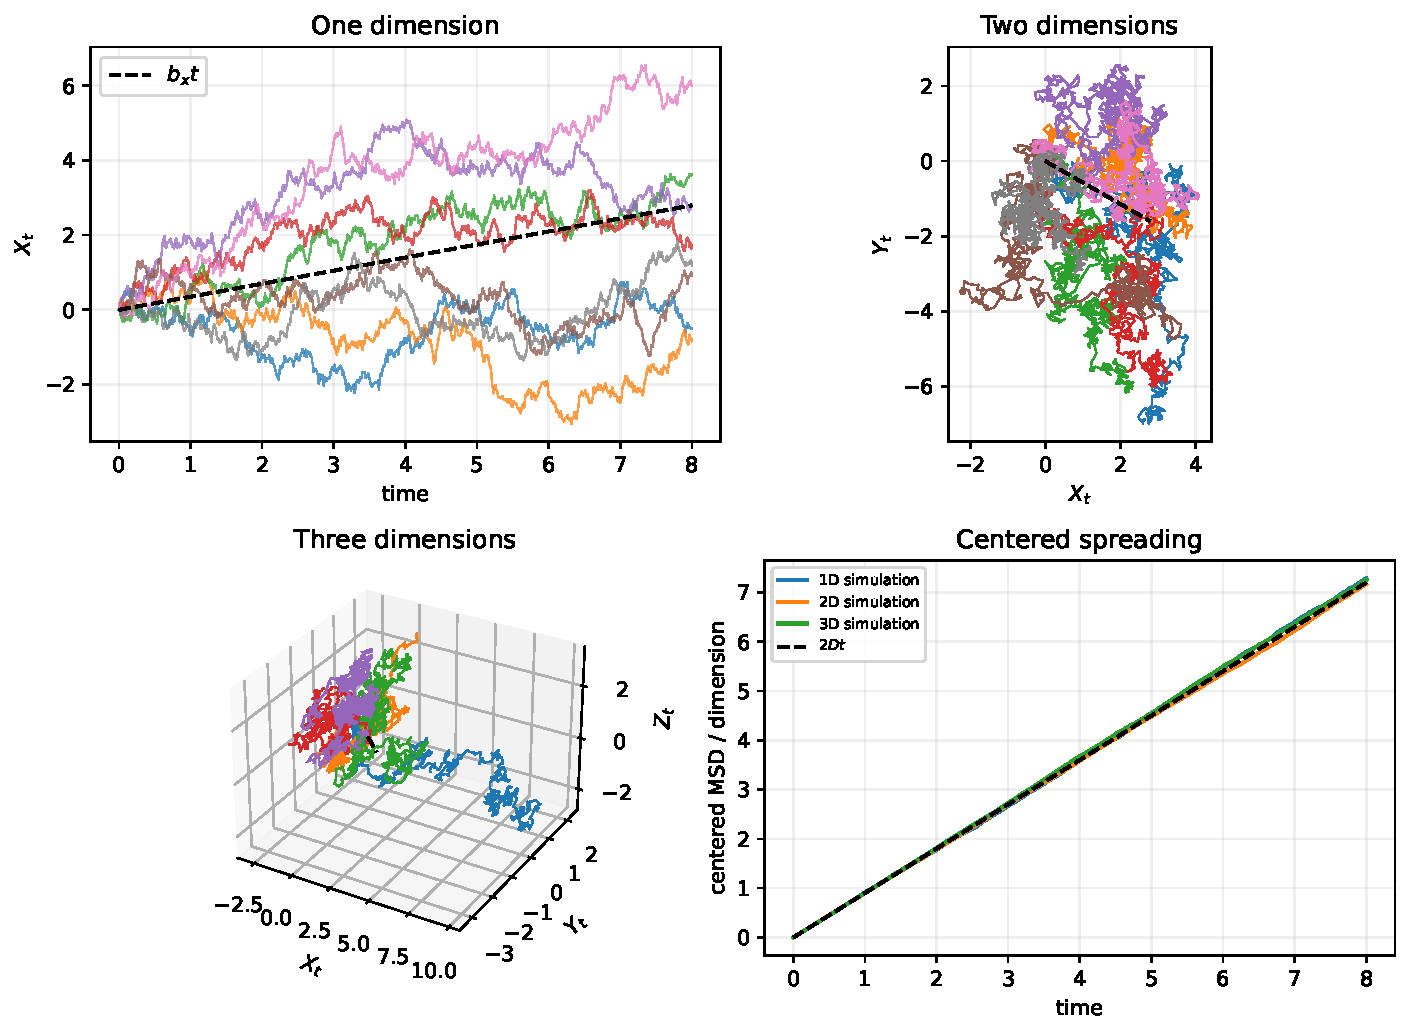
\includegraphics[width=\textwidth]
    {figures/08_brownian-motion-diffusion/06-euler-maruyama-drift-diffusion.pdf}
  \caption{Euler--Maruyama simulations of drift--diffusion in one, two, and
  three dimensions.  Individual paths fluctuate around the ensemble drift,
  while the centered covariance grows according to the prescribed diffusion
  tensor.\figurenotebookmark}
  \label{fig:transport-euler-maruyama}
\end{figure}
\footnotetext{\textit{Student reproduction notebook:}
  \href{run:figures/08_brownian-motion-diffusion/06-euler-maruyama-drift-diffusion.ipynb}
  {\texttt{06: Euler--Maruyama drift--diffusion}}.}

\section{From stochastic paths to an ensemble equation}

Let $P(\bm r,t)$ denote the probability density of
\cref{eq:transport-general-sde}.  The adjoint of the It\^o generator gives the
Fokker--Planck equation
\begin{equation}
  \frac{\partial P}{\partial t}
  =-\sum_i\frac{\partial}{\partial x_i}(b_iP)
  +\sum_{ij}\frac{\partial^2}{\partial x_i\partial x_j}(D_{ij}P).
  \label{eq:transport-fokker-planck-general}
\end{equation}
For constant isotropic $D$,
\begin{equation}
  \frac{\partial P}{\partial t}
  =-\nabla\cdot(\bm bP)+D\nabla^2P.
  \label{eq:transport-fokker-planck-isotropic}
\end{equation}
Writing this equation as a conservation law identifies the probability current:
\begin{equation}
  \frac{\partial P}{\partial t}+\nabla\cdot\bm J_P=0,
  \qquad
  \boxed{\bm J_P=\bm bP-D\nabla P.}
  \label{eq:transport-probability-current}
\end{equation}
The current contains advective transport with the drift and diffusive transport
down the density gradient.

A point source containing $N_0$ particles in an infinite isotropic medium has
the density
\begin{equation}
  n(\bm r,t)
  =\frac{N_0}{(4\pi Dt)^{d/2}}
   \exp\!\left(-\frac{|\bm r|^2}{4Dt}\right).
  \label{eq:transport-diffusion-green-function}
\end{equation}
Its spatial integral is $N_0$, its mean position is zero, and its mean-square
radius is $2dDt$.  These three relations test normalization, symmetry, and the
diffusive width independently.

\section{The master equation and Fick's law}

The continuum equation also follows directly from a lattice walk.  Let $P_i^N$
be the probability at $x_i=i\ell$ after $N$ steps.  Nearest-neighbor motion
gives
\begin{equation}
  P_i^{N+1}=\frac12P_{i-1}^N+\frac12P_{i+1}^N.
  \label{eq:transport-master-equation}
\end{equation}
Subtracting $P_i^N$, dividing by $\Delta t$, and using
\cref{eq:transport-random-walk-diffusivity} yields
\begin{equation}
  \frac{P_i^{N+1}-P_i^N}{\Delta t}
  =D\frac{P_{i+1}^N-2P_i^N+P_{i-1}^N}{\ell^2}.
  \label{eq:transport-master-centered}
\end{equation}
The continuum limit is
\begin{equation}
  \boxed{\frac{\partial P}{\partial t}=D\frac{\partial^2P}{\partial x^2}.}
  \label{eq:transport-diffusion-equation-probability}
\end{equation}

The same crossing count produces the constitutive flux.  If $n_i$ is a
one-dimensional number density, the expected signed particle current through
the face between cells $i$ and $i+1$ is
\begin{equation}
  \Gamma_{i+1/2}
  =\frac{\ell}{2\Delta t}(n_i-n_{i+1}).
  \label{eq:transport-discrete-face-flux}
\end{equation}
For a slowly varying density,
$n_{i+1}-n_i=\ell\,\partial_xn+\mathcal O(\ell^2)$, so
\begin{equation}
  \boxed{\bm\Gamma=-D\nabla n.}
  \label{eq:transport-ficks-law}
\end{equation}
This is Fick's first law.  Its sign states that the net particle flux points
down the density gradient.

Local conservation of particle number is
\begin{equation}
  \frac{\partial n}{\partial t}+\nabla\cdot\bm\Gamma=S,
  \label{eq:transport-number-continuity}
\end{equation}
where $S$ is the net volumetric source rate.  For $S=0$, substitution of
\cref{eq:transport-ficks-law} gives
\begin{equation}
  \boxed{
  \frac{\partial n}{\partial t}
  =\nabla\cdot(D\nabla n).
  }
  \label{eq:transport-ficks-second-law}
\end{equation}
If $D$ is uniform, this reduces to
$\partial_tn=D\nabla^2n$.  A spatially varying $D$ remains inside the
divergence.  Replacing $\nabla\cdot(D\nabla n)$ by $D\nabla^2n$ would omit
$(\nabla D)\cdot\nabla n$.

\section{The heat equation}

Let $u$ be thermal energy per unit volume and $\bm j_Q$ the heat flux.  Energy
conservation without volumetric heating is
\begin{equation}
  \frac{\partial u}{\partial t}+\nabla\cdot\bm j_Q=0.
  \label{eq:transport-energy-continuity}
\end{equation}
Fourier's law is
\begin{equation}
  \bm j_Q=-\kappa\nabla T,
  \label{eq:transport-fourier-law}
\end{equation}
where $\kappa$ is thermal conductivity.  With approximately constant volumetric
heat capacity $C_V$, $u=C_VT$, and therefore
\begin{equation}
  C_V\frac{\partial T}{\partial t}
  =\nabla\cdot(\kappa\nabla T).
  \label{eq:transport-general-heat-equation}
\end{equation}
Uniform $C_V$ and $\kappa$ give
\begin{equation}
  \boxed{
  \frac{\partial T}{\partial t}=\alpha\nabla^2T,
  \qquad
  \alpha=\frac{\kappa}{C_V}.
  }
  \label{eq:transport-heat-equation}
\end{equation}
The heat equation and particle diffusion equation share a mathematical
operator.  Their fields, fluxes, constitutive coefficients, and conserved
quantities remain distinct.  Thermal conductivity $\kappa$, electrical
conductivity $\sigma$, particle diffusivity $D$, and thermal diffusivity
$\alpha$ are not interchangeable.

\section{Matrix representation and exponential evolution}

Consider $M$ periodic cells of width $h$.  Define the incidence matrix $B$ so
that row $i$ computes $f_{i+1}-f_i$, with the final row wrapping to the first
cell.  The discrete gradient is
\begin{equation}
  G=\frac{B}{h}.
  \label{eq:transport-discrete-gradient}
\end{equation}
For particle diffusion, the face flux and finite-volume balance are
\begin{equation}
  \bm\Gamma=-DG\bm n,
  \qquad
  \frac{\dd\bm n}{\dd t}=\frac1hB^{\mathsf T}\bm\Gamma.
  \label{eq:transport-discrete-flux-continuity}
\end{equation}
Combining them gives
\begin{equation}
  \frac{\dd\bm n}{\dd t}=D L\bm n,
  \qquad
  \boxed{L=-\frac{B^{\mathsf T}B}{h^2}.}
  \label{eq:transport-matrix-diffusion}
\end{equation}
The factorization shows that $L$ is symmetric and negative semidefinite.  Its
constant eigenvector has eigenvalue zero because periodic diffusion conserves
the spatial sum.

Let
\begin{equation}
  L=V\Lambda V^{\mathsf T},
  \qquad
  V^{\mathsf T}V=I.
  \label{eq:transport-laplacian-eigendecomposition}
\end{equation}
The exact semidiscrete solution is
\begin{equation}
  \boxed{
  \bm n(t)=e^{DLt}\bm n(0)
  =V e^{D\Lambda t}V^{\mathsf T}\bm n(0).
  }
  \label{eq:transport-matrix-exponential}
\end{equation}
Every negative eigenvalue produces exponential decay.  The zero eigenvalue
preserves the mean.  The propagator satisfies
\begin{equation}
  e^{DL(t+s)}=e^{DLt}e^{DLs}.
  \label{eq:transport-semigroup}
\end{equation}

The explicit-Euler update is
\begin{equation}
  \bm n^{r+1}=(I+D\Delta t L)\bm n^r.
  \label{eq:transport-explicit-euler}
\end{equation}
For the centered one-dimensional Laplacian, stability requires
$D\Delta t/h^2\leq1/2$.  The exponential propagator has no corresponding
step-size stability restriction.  Dense diagonalization serves small teaching
problems; large sparse systems require Krylov, implicit, or operator-splitting
methods.

Boundary conditions alter both conservation and the spectrum.  Periodic and
zero-flux boundaries preserve the total amount in a closed domain.  Fixed-value
boundaries exchange particles or energy with a reservoir.  Absorbing particle
boundaries remove probability from the modeled domain.

\begin{figure}[htbp]
  \centering
  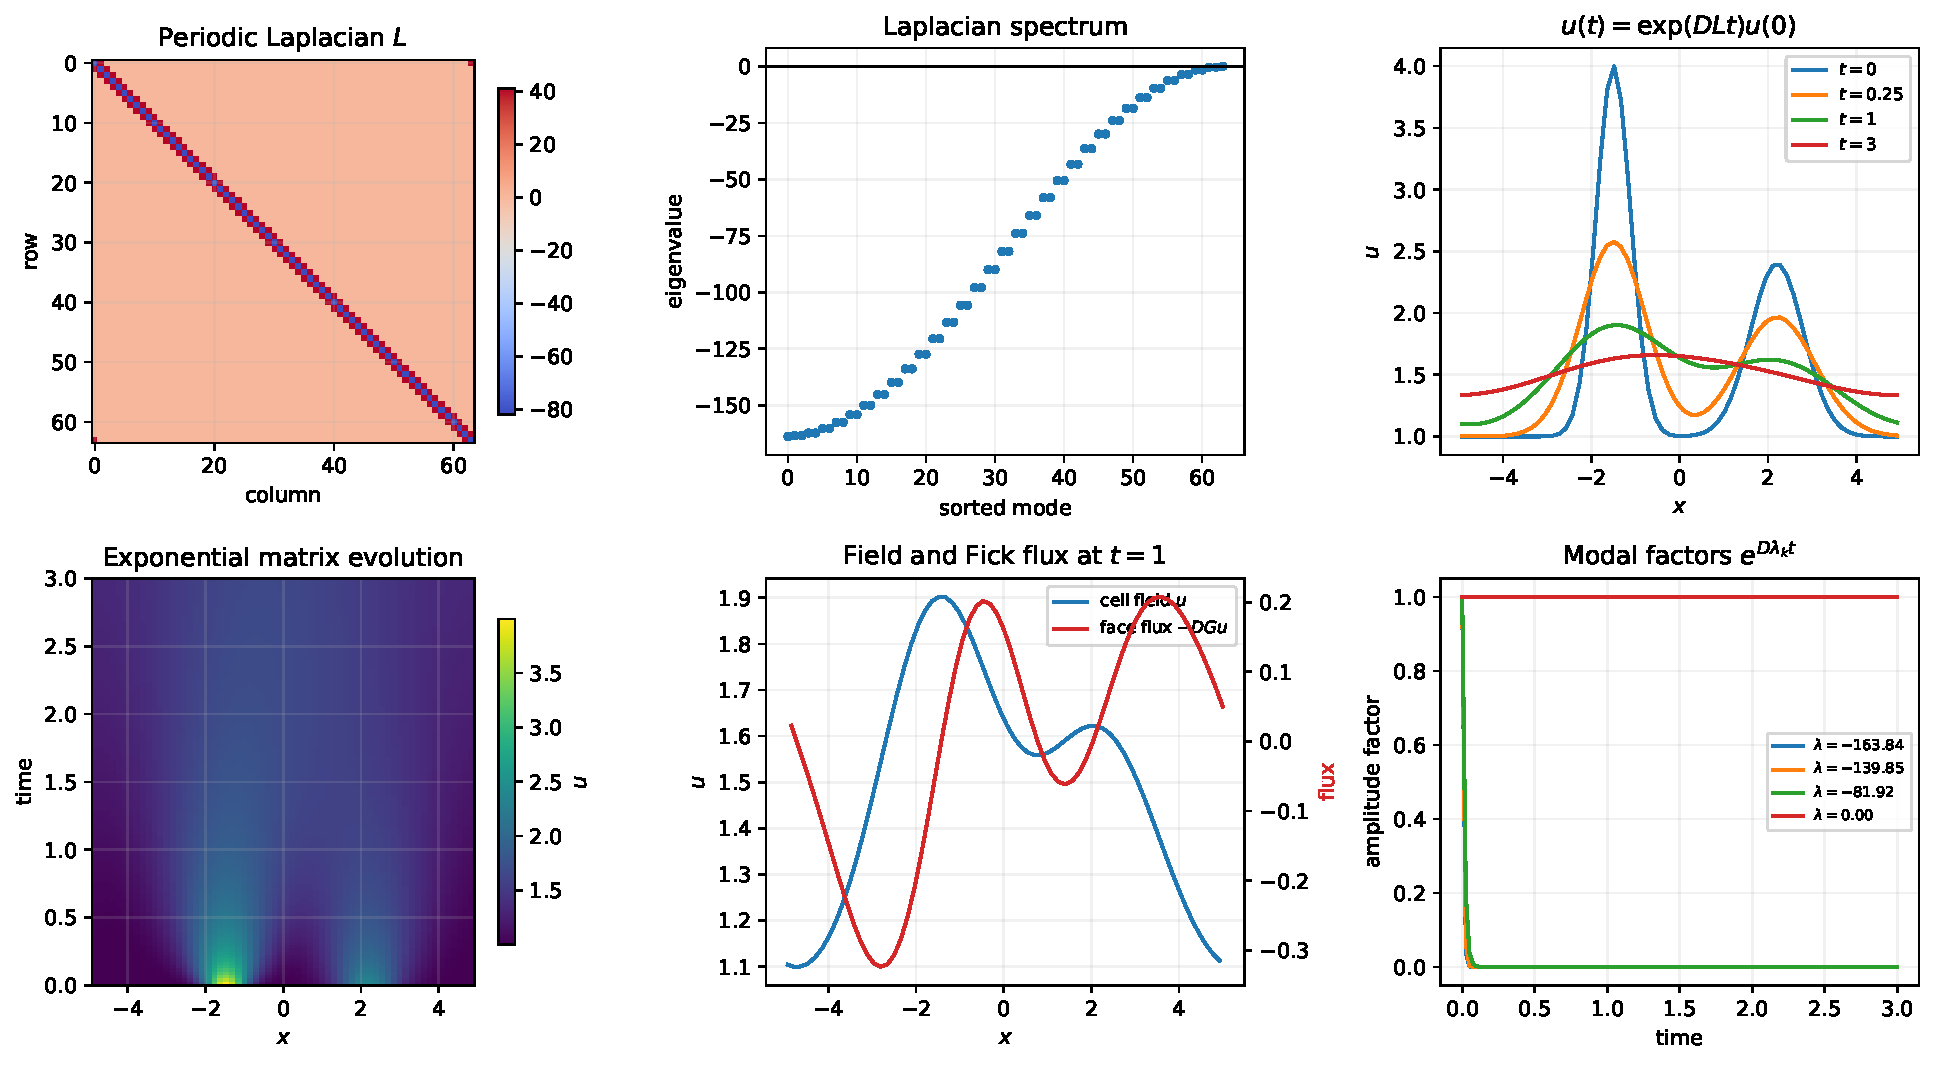
\includegraphics[width=\textwidth]
    {figures/08_brownian-motion-diffusion/lab-03-matrix-diffusion-exponential-evolution.pdf}
  \caption{Matrix representation of periodic diffusion.  The Laplacian
  spectrum is nonpositive, nonuniform modes decay exponentially, the constant
  mode is conserved, and the face flux follows from the discrete
  gradient.\figurenotebookmark}
  \label{fig:transport-matrix-exponential}
\end{figure}
\footnotetext{\textit{Student reproduction notebook:}
  \href{run:figures/08_brownian-motion-diffusion/lab-03-matrix-diffusion-exponential-evolution.ipynb}
  {\texttt{Lab 3: matrix diffusion and exponential evolution}}.}

The calculation in \cref{fig:transport-matrix-exponential} constructs a
$64\times64$ periodic Laplacian with 192 nonzero entries.  Its eigenvalues lie
in $[-163.84,0]$ to numerical precision.  The conserved-integral drift is below
$3.2\times10^{-14}$, and the matrix-exponential semigroup error is approximately
$1.1\times10^{-15}$ in the infinity norm.

The same discrete Laplacian appears in a free-particle Hamiltonian,
\begin{equation}
  H=-\frac{\hbar^2}{2m}L.
  \label{eq:transport-free-hamiltonian}
\end{equation}
A Laplacian eigenvalue $\lambda_j\leq0$ produces the quantum multiplier
$\exp[-\mathrm iE_jt/\hbar]$, whose magnitude is one, and the diffusive
multiplier $\exp(D\lambda_jt)$, which decays for $\lambda_j<0$.  The spatial
modes are identical; the evolution laws are not.

\section{Range of validity}

The diffusion equation is a continuum closure.  It applies when the modeled
length is large compared with the microscopic step length and the modeled time
is long compared with the velocity-memory time.  Constant scalar diffusivity
assumes an isotropic, homogeneous medium.  Ballistic motion, correlated steps,
spatially varying materials, and anomalous waiting-time statistics require a
kinetic, tensor, or non-Fickian description.

\section{Chapter summary}

Independent microscopic steps produce a mean-square displacement proportional
to time.  Their continuum limit is Brownian motion, whose ensemble density
obeys the Fokker--Planck equation.  Signed crossing counts produce Fick's law,
and local conservation converts that constitutive law into the diffusion
equation.  Fourier's law gives the heat equation with the same Laplacian but a
different physical field and coefficient.  Spatial discretization yields
$\dot{\bm f}=\chi L\bm f$, with exact semidiscrete evolution
$\bm f(t)=e^{\chi Lt}\bm f(0)$.  The next chapter restores the velocity degree
of freedom and derives the Maxwell--Boltzmann gas from underdamped Langevin
dynamics.
